\section{PRUEBAS EN SIMULADOR} \label{pruebas-simulador}
% rendimiento en simulacion (imágenes con giros y sus predicciones),
% gráfica del EMA.
% Casos de predicciones correctas vs erroneas en calles.
% Casos de predicciones correctas vs erroneas en intersecciones.
Una vez se tiene la certeza del funcionamiento del modelo mediante el análisis de sus métricas de error, se comprueban los resultados empíricamente con simulaciones en el ambiente virtual de la ciudad de CARLA.
\subsection{CONDUCCIÓN}
Ya se revisaron los resultados de segmentación, estimación de distancias y clasificación de objetos en la imagen, luego de pasar por todas las etapas descritas del modelo, las salidas obtenidas son el valor del giro y la aceleración.

\begin{figure}[H]
	\centering
	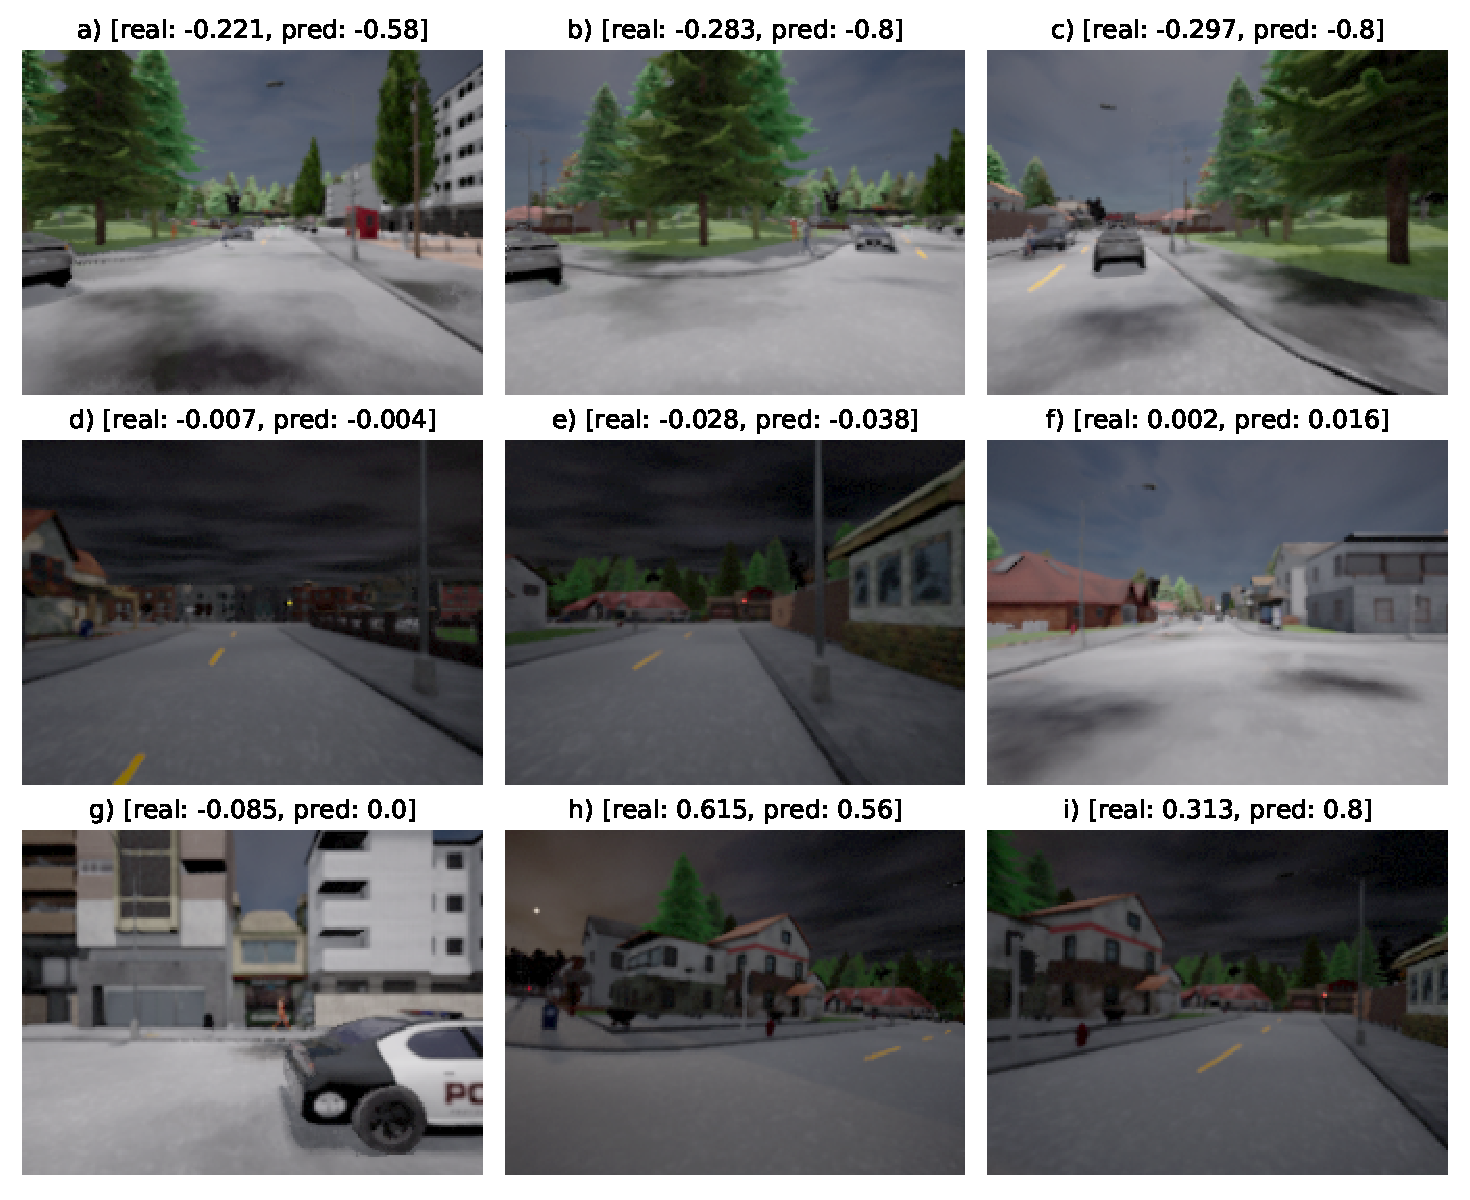
\includegraphics[scale=0.63]{imagenes/preds/steer}
	\caption[Comparación de Dirección Real y Estimada]{comparación de dirección real y estimada}
	\label{steer}
\end{figure}

Comparando las predicciones en distintas situaciones se tienen los resultados de la figura \ref{steer}, de la cual se puede observar en los casos $a, b, c, h, i$, los cuales consisten en giros durante intersecciones, que el modelo es mucho más agresivo al tomar las curvas, aplicando un giro mayor de la dirección. En el caso $f$ que es una intersección en la cual se decide seguir recto, predice correctamente no girar. En la situación de la imagen $g$, se tiene una casi colisión con otro vehículo, en cuyo caso la predicción es 0, al igual que la aceleración, y finalmente en las imágenes $d$ y $e$ no existe mucha variación del $0$ ya que se encuentra en una recta dentro de su carril.

\subsection{FALLOS}
A pesar del buen rendimiento del modelo en las situaciones de prueba, siempre existe un margen de error contemplado en las métricas evaluadas, así se presentan situaciones puntuales donde el vehículo se detiene abruptamente al confundir charcos de agua en la vía con vehículos cercanos (figura \ref{charco}), o los más graves cuando se sale del camino y colisiona con objetos en las aceras \ref{colision}.

\begin{figure}[H]
	\centering
	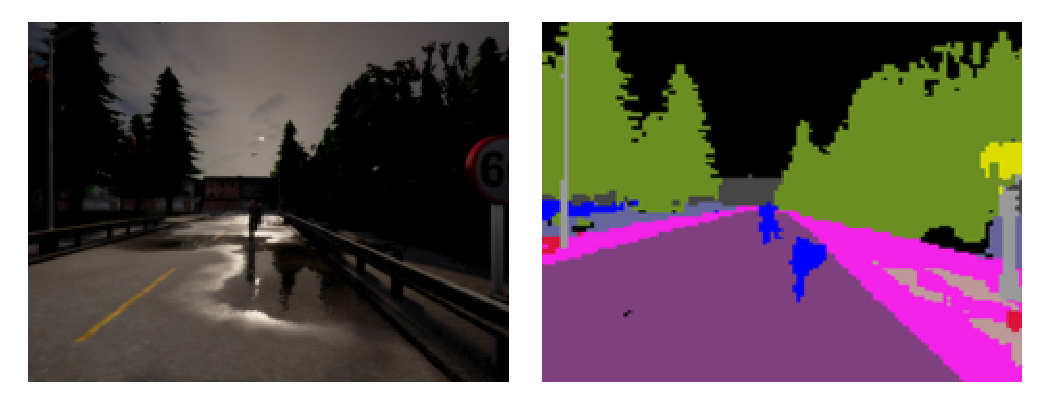
\includegraphics[scale=0.7]{imagenes/preds/err1}
	\caption[Charco erroneamente Clasificado]{Charco erroneamente Clasificado}
	\label{charco}
\end{figure}

%\begin{figure}[H]
%	\centering
%	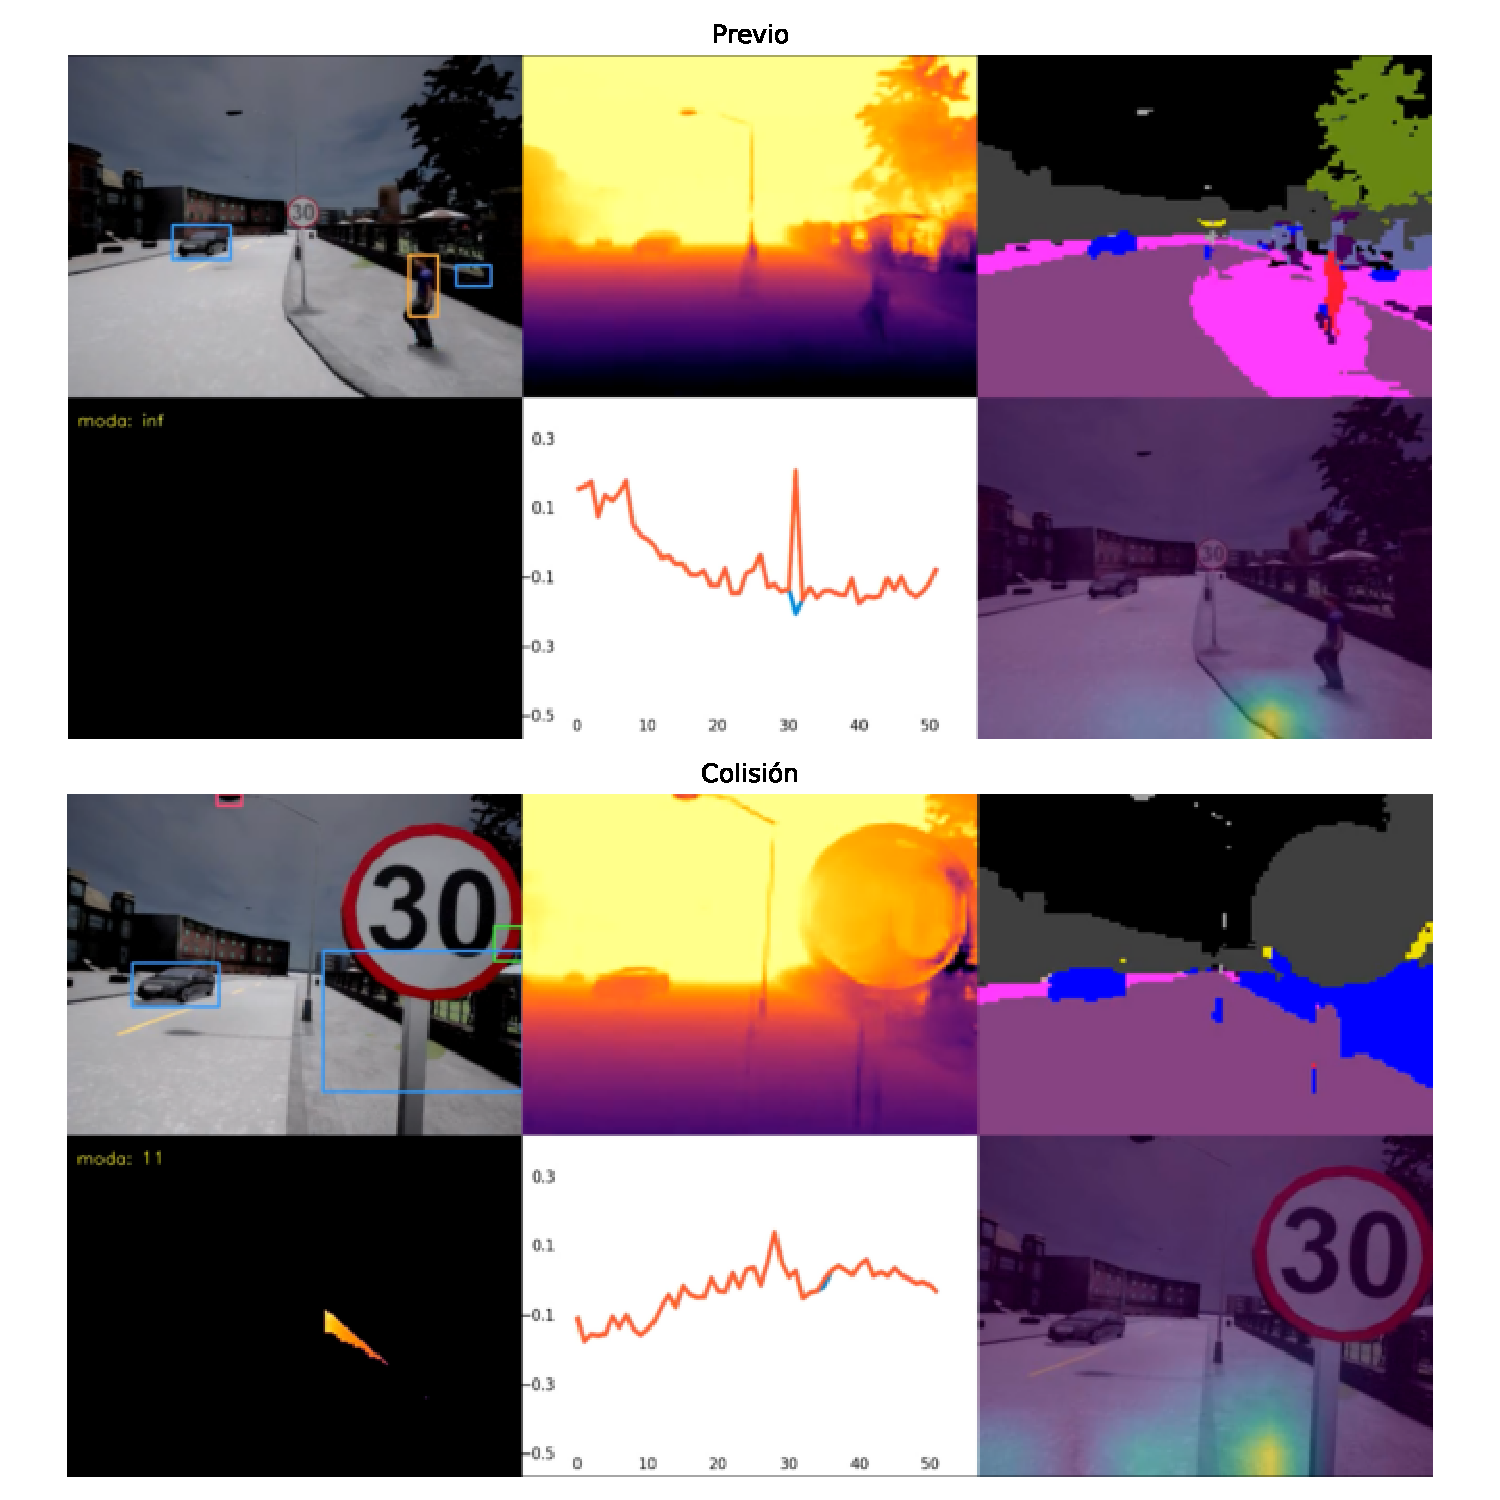
\includegraphics[scale=0.6]{imagenes/preds/err2}
%	\caption[Colisión con Poste]{colisión con poste}
%	\label{colision}
%\end{figure}

En la figura \ref{colision} se nota que la segmentación falla al no detectar el poste como obstáculo lo cual deriva en que no se calcule la distancia a este y se produzca la colisión.

\begin{figure}[H]
	\centering
	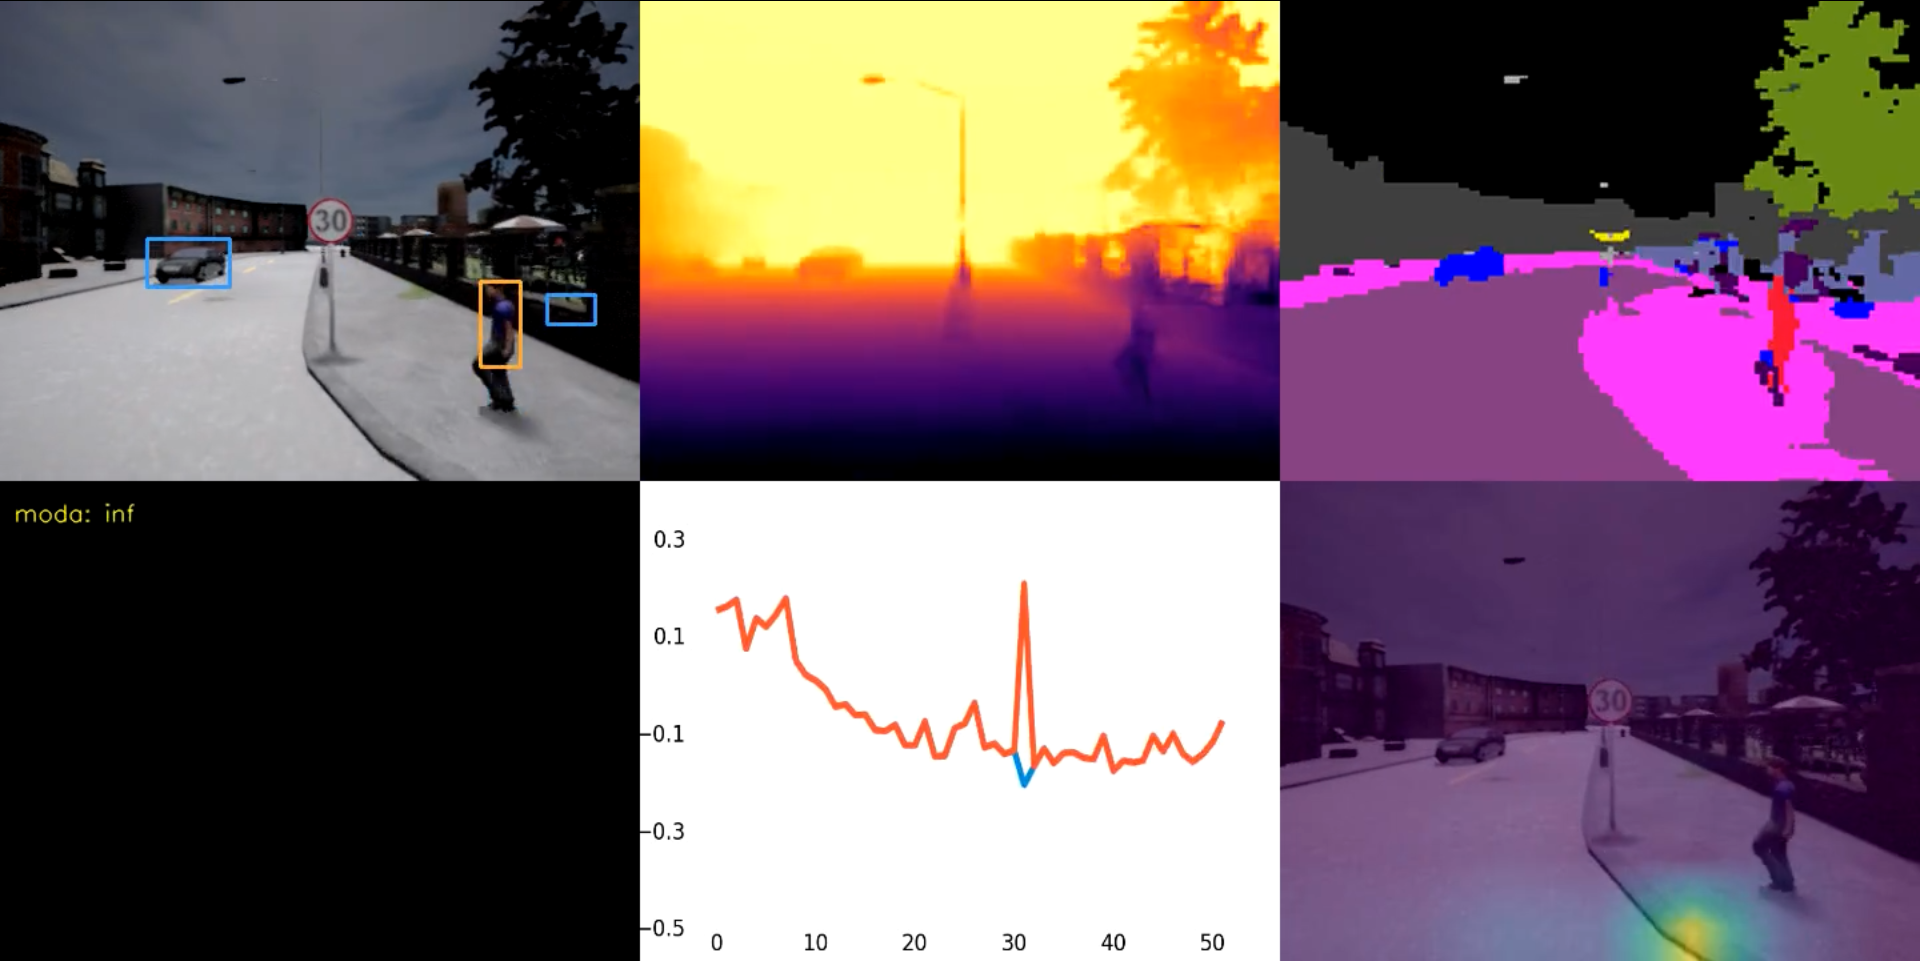
\includegraphics[scale=0.22]{imagenes/preds/crash1}
\end{figure}

\begin{figure}[H]
	\centering
	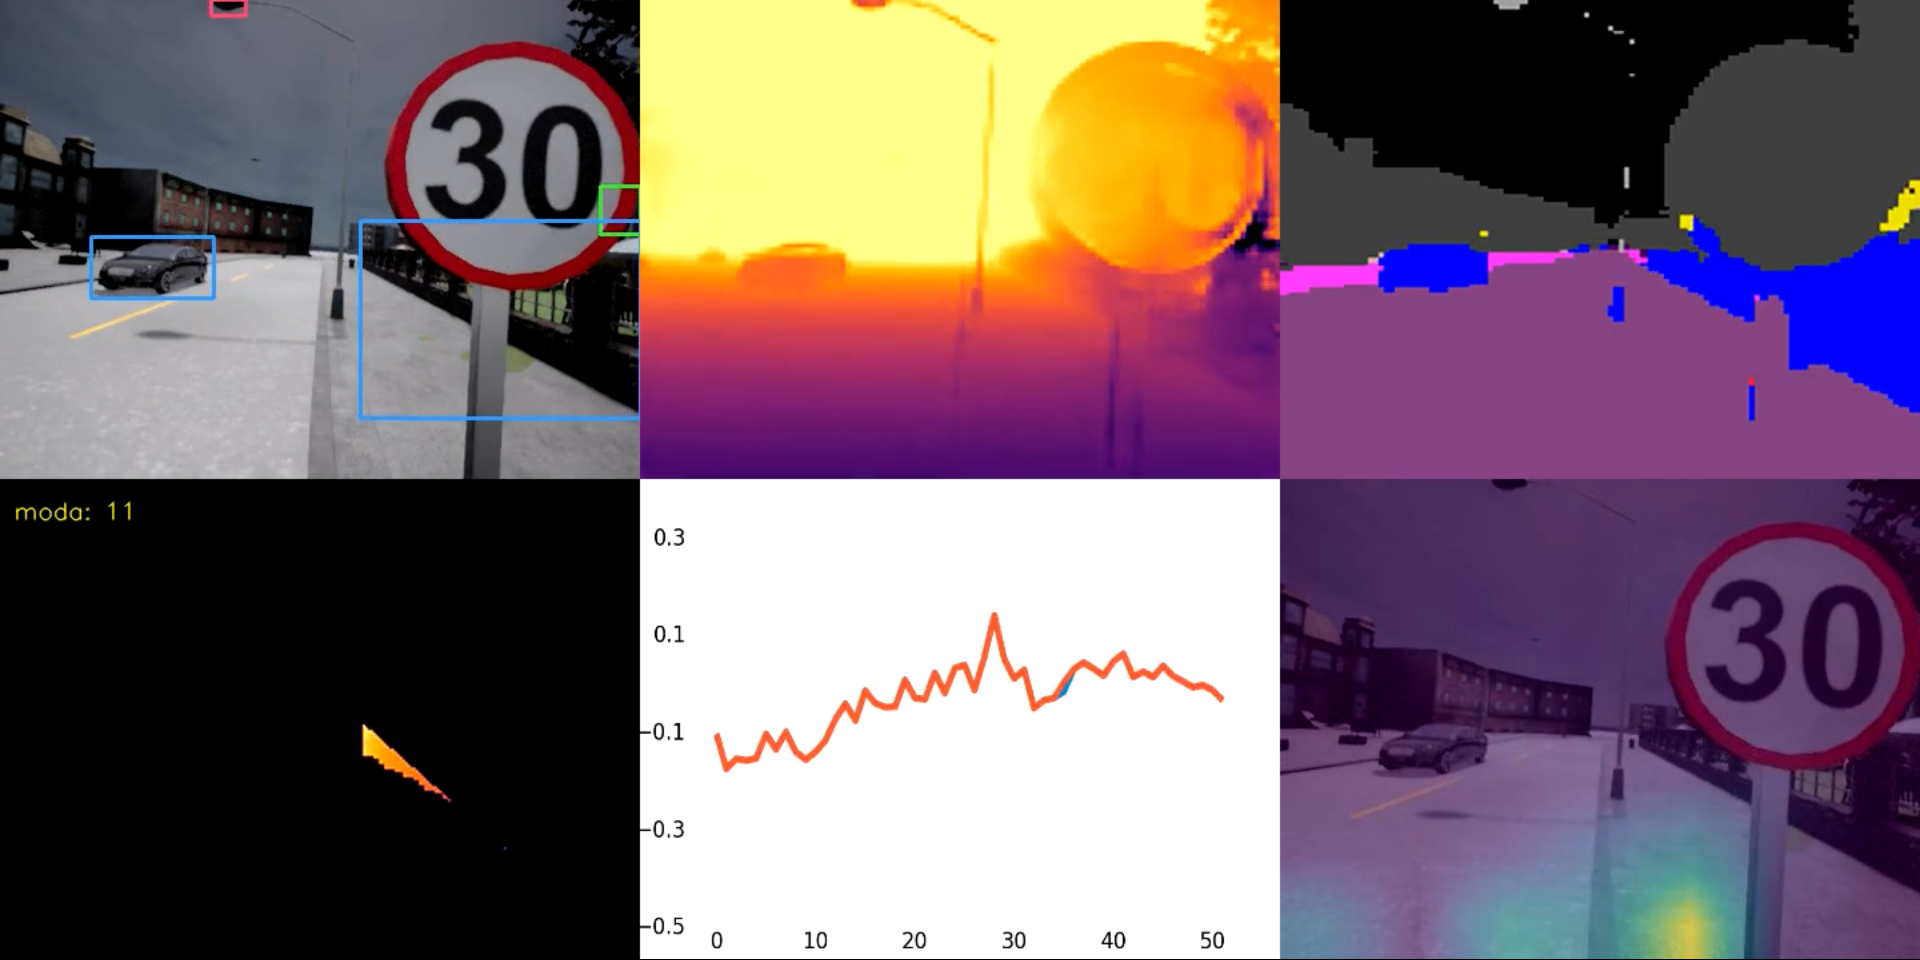
\includegraphics[scale=0.22]{imagenes/preds/crash2}
	\caption[Colisión con Poste]{colisión con poste}
	\label{colision}
\end{figure}

En total se realizaron 17 simulaciones de prueba de las cuales en 3 se cometieron errores, los cuales fueron confundir un charco como vehículo, frenando totalmente y no reanudando la marcha,  el de salirse del camino sin detectar un poste, colisionando así contra él, y el de invadir un carril en contra ruta frenando para no colisionar y congestionando el tráfico ya que no puede dar marcha atrás.